\documentclass[unicode,12pt]{beamer}
\usepackage{luatexja}
\usepackage[hiragino-pro]{luatexja-preset}
\usepackage{luatexja-fontspec}
\renewcommand{\kanjifamilydefault}{\gtdefault}

\setmonofont{x14y24pxHeadUpDaisy}
\newfontfamily{\magnolia}{Magnolia Script}
\newfontfamily{\brush}{Brush Script MT}

\usepackage{luatexja-ruby}
\usepackage{url}
\usepackage{listings}

\lstdefinelanguage{dhall}{
  keywords={let, in},
  keywordstyle=\color{main}\bfseries,
  keywords=[2]{Bool, Integer, Double, Text, List, Optional},
  keywordstyle=[2]\color{accent}\bfseries,
  identifierstyle=\color{text},
  sensitive=false,
  comment=[l]{--},
  %morecomment=[s]{{-}{-}},
  commentstyle=\color{subtext}\ttfamily,
  stringstyle=\color{main}\ttfamily,
  morestring=[b]',
  morestring=[b]"
}

\lstdefinelanguage{yaml}{
  keywords={let, in},
  keywordstyle=\color{main}\bfseries,
  identifierstyle=\color{text},
  sensitive=false,
  comment=[l]{--},
  %morecomment=[s]{{-}{-}},
  commentstyle=\color{subtext}\ttfamily,
  stringstyle=\color{main}\ttfamily,
  morestring=[b]',
  morestring=[b]"
}

\lstset{
   language=dhall,
   extendedchars=true,
   basicstyle=\footnotesize\ttfamily,
   showstringspaces=false,
   showspaces=false,
   tabsize=2,
   breaklines=true,
   showtabs=false
}

\definecolor{main}{RGB}{49,118,137}
\definecolor{accent}{RGB}{220,94,74}
\definecolor{text}{RGB}{50,50,50}
\definecolor{subtext}{RGB}{80,80,80}

\usetheme{Copenhagen}
\usecolortheme{beaver}
\setbeamertemplate{footline}[page number]

\setbeamercolor{alerted text}{fg=accent}
\setbeamercolor{background canvas}{bg=white}
\setbeamercolor{block body alerted}{bg=normal text.bg!90!black}
\setbeamercolor{block body}{bg=normal text.bg!90!black}
\setbeamercolor{block body example}{bg=normal text.bg!90!black}
\setbeamercolor{block title alerted}{use={normal text,alerted text},fg=alerted text.fg!75!normal text.fg,bg=normal text.bg!75!black}
\setbeamercolor{block title}{bg=main}
\setbeamercolor{block title example}{use={normal text,example text},fg=example text.fg!75!normal text.fg,bg=normal text.bg!75!black}
\setbeamercolor{fine separation line}{}
\setbeamercolor{frametitle}{fg=main}
\setbeamercolor{item projected}{fg=subtext}
\setbeamercolor{normal text}{fg=subtext}
\setbeamercolor{palette sidebar primary}{use=normal text,fg=normal text.fg}
\setbeamercolor{palette sidebar quaternary}{use=structure,fg=structure.fg}
\setbeamercolor{palette sidebar secondary}{use=structure,fg=structure.fg}
\setbeamercolor{palette sidebar tertiary}{use=normal text,fg=normal text.fg}
\setbeamercolor{section in sidebar}{fg=brown}
\setbeamercolor{section in sidebar shaded}{fg=grey}
\setbeamercolor{separation line}{}
\setbeamercolor{sidebar}{bg=red}
\setbeamercolor{sidebar}{parent=palette primary}
\setbeamercolor{structure}{bg=white, fg=main}
\setbeamercolor{subsection in sidebar}{fg=brown}
\setbeamercolor{subsection in sidebar shaded}{fg=grey}
\setbeamercolor{title}{fg=main}
\setbeamercolor{titlelike}{fg=main}

\newlength{\mytotalwidth}
\mytotalwidth=\dimexpr\linewidth-5mm
\newlength{\mycolumnwidth}
\mycolumnwidth=\dimexpr\mytotalwidth-5mm

\title{並列並行言語Haskell}
\author[@syocy]{
    \frame{
\includegraphics[width=1cm]{icon.jpg}}\\%
    \vspace{0.5em}%
    @syocy%
}

%\institute{Engineering team}
\date{2018-11-10}

\begin{document}

\begin{frame}[plain]\frametitle{}
  \titlepage
\end{frame}

\section{}

\begin{frame}[plain]{参考書}
  \centering
  Haskellによる並列・並行プログラミング
  (写真)
\end{frame}

\section{並列・並行の動向}

\begin{frame}{プロセッサ性能トレンド}
  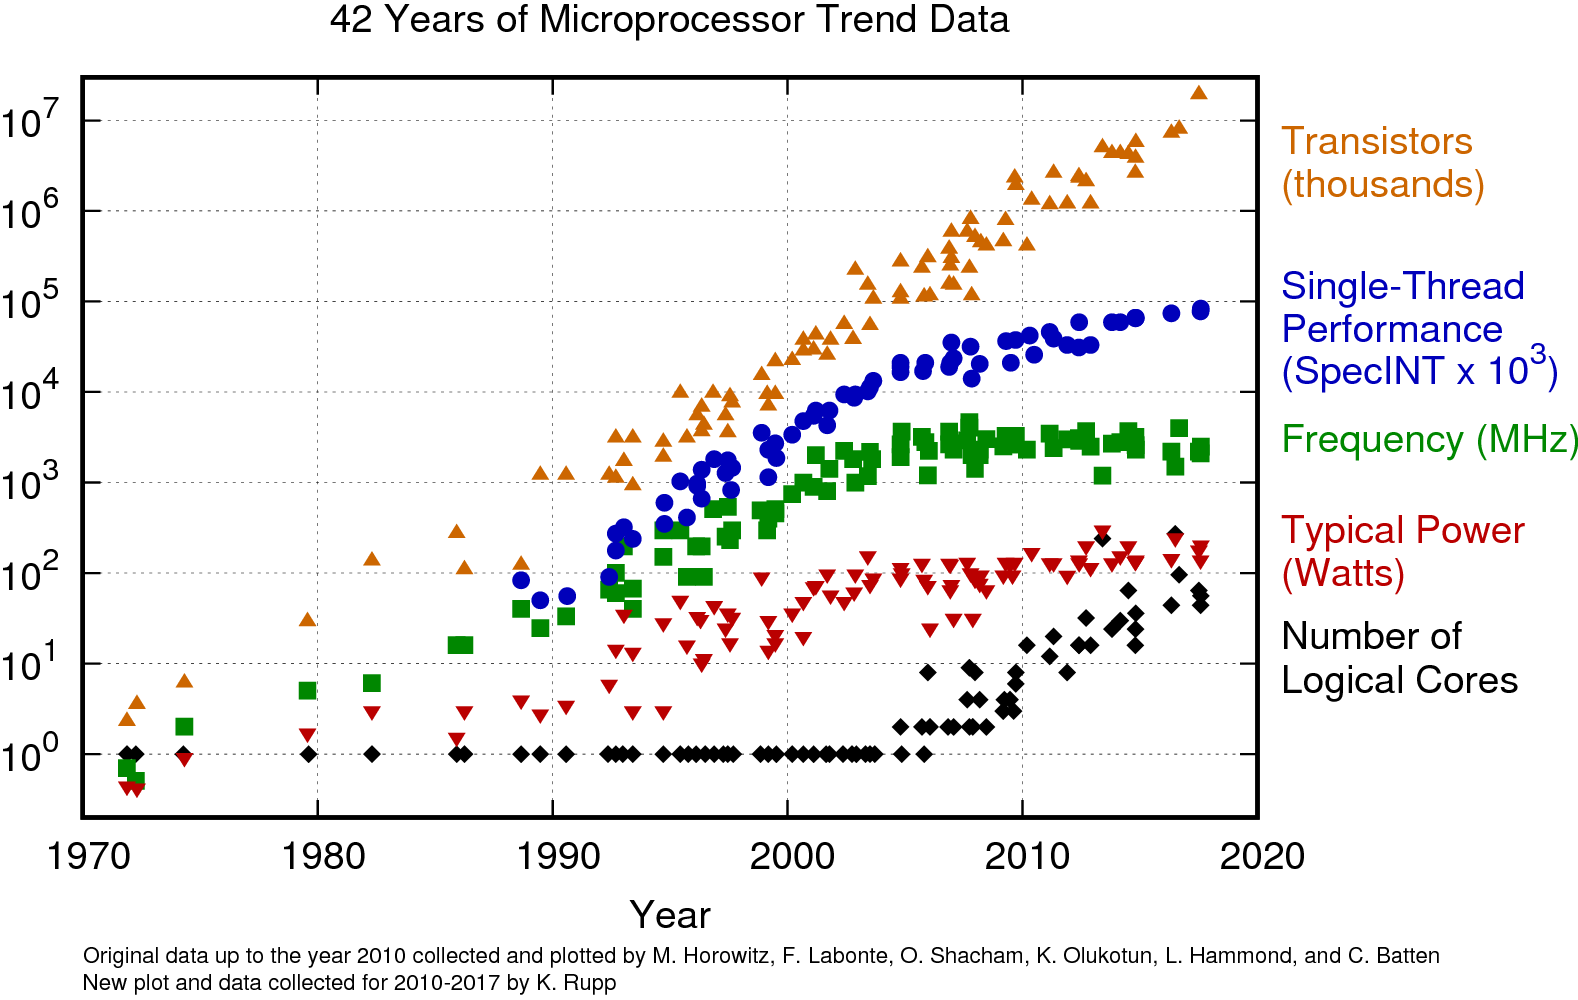
\includegraphics[width=\textwidth]{pic/42-years-processor-trend.png}
\end{frame}

\begin{frame}{プロセッサ性能トレンド}
  \begin{columns}[totalwidth=\mytotalwidth]
    \begin{column}[T]{0.3\mycolumnwidth}
      \centering
      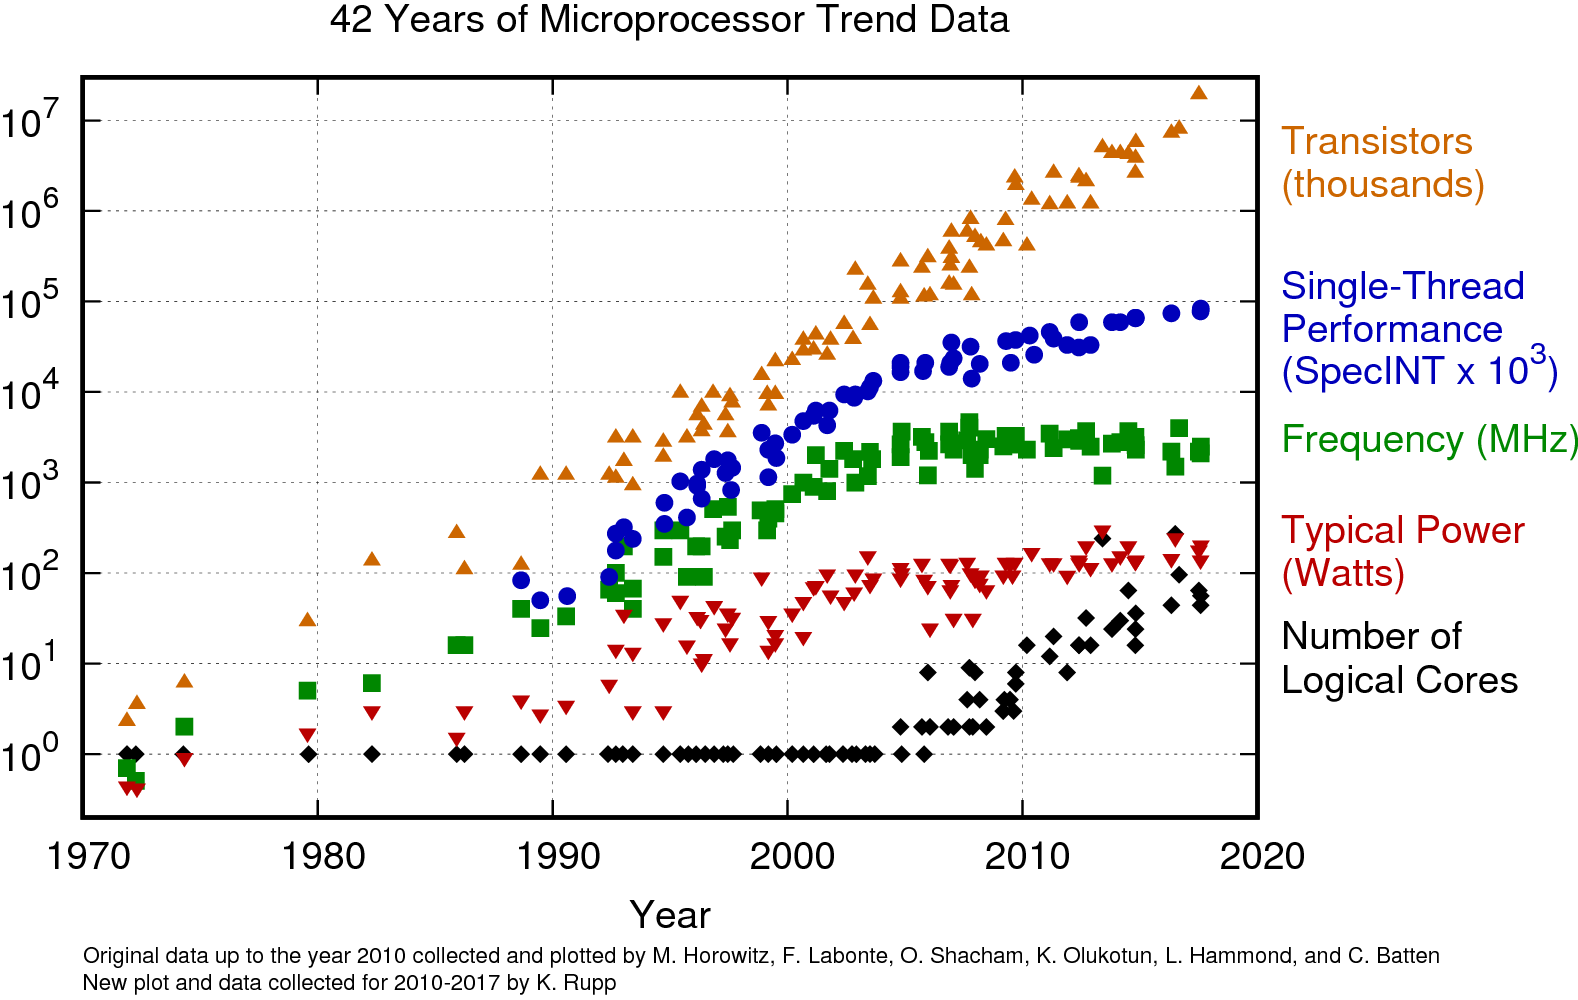
\includegraphics[width=\columnwidth]{pic/42-years-processor-trend.png}
    \end{column}
    \begin{column}[t]{0.7\mycolumnwidth}
      \begin{itemize}
      \item シングルスレッド性能は伸び悩んできている
      \item 一方で論理コア数は順調に増えてきている
      \item \alert{現代のプロセッサの能力を引き出すにはコア数を活かすプログラミングが必要}
      \end{itemize}
    \end{column}
  \end{columns}
\end{frame}

\begin{frame}{お求めやすくなったメニーコアCPU}
  \begin{itemize}
  \item 10以上\footnote{メニーコアの定義は曖昧。ここでは物理10コア以上をメニーコアと呼ぶことにする。}
    の物理コアを持つCPUがご家庭でも手に入れられるお値段になった
    \end{itemize}
  \begin{tabular}{llll} \hline
    CPU & Core & Freq & Price\footnote{価格は変動します} \\ \hline
    Ryzen TR 2990WX & 32-core 64-thread & 3.00GHz & \$1799 \\
    Ryzen TR 2950X & 16-core 32-thread & 3.50GHz & \$899 \\
    Ryzen TR 1920X & 12-core 24-thread & 3.5GHz & \$399 \\
    \hline
  \end{tabular}
\end{frame}

\begin{frame}{並列並行言語の台頭}
  最近話題の言語はコアな部分に並列並行機能を備えていることが多い \\
  → 並列並行の重要性が意識され始めた
  \begin{itemize}
  \item Go: goroutine(軽量スレッド)を持つ
  \item Erlang, Elixir: VMが軽量プロセスを持つ
  \item Rust: メモリー安全性が並行性にも及ぶことを強調している
  \end{itemize}
  Haskell はどうか?
\end{frame}

\section{並列・並行とHaskell}

\begin{frame}{並列・並行とHaskell}
  Haskell (GHC) は古くから並列・並行を考えて設計されてきた
  \begin{itemize}
  \item 1997年にライブラリではなく実行時システムとして並行性をサポートすることが決定
  \item 2004年に実行時システムを共有メモリのマルチプロセッサ上で並列に動作させることが決定
  \item 2009年の論文 ``Runtime support for multicore Haskell''
  \end{itemize}
\end{frame}

\begin{frame}{並列・並行のためのよい性質}
  Haskell は並列・並行のためのよい特徴を持つ
  \begin{itemize}
  \item Haskell は純粋なコードと副作用(IOなど)を含むコードを分離できる
    \begin{itemize}
    \item 並列性は\alert{決定的}: 並列度や実行環境が変わろうと結果は変わらない
    \end{itemize}
  \item 実行時システムが\alert{軽量スレッド}をサポートする
    \begin{itemize}
    \item よく並行性の実現にはスレッドが用いられるが、
    \item あたかも普通の(OS)スレッドのように使えるものが、普通のスレッドよりはるかに軽く動作する
    \end{itemize}
  \end{itemize}
  Haskell 使うっきゃない!
\end{frame}

\section{並列・並行(・分散)の意味}

\begin{frame}{並列・並行(・分散)って?}
  これまで断りなく使ってきた言葉
  \begin{itemize}
  \item 並列(parallel)
  \item 並行(concurrent)
  \item (分散(distributed))
  \end{itemize}
  に違いはあるの?
\end{frame}

\begin{frame}{目的による分類}
  並列と並行には異なる目的がある
  \begin{itemize}
  \item 並列(parallel): 複数の情報処理ユニットを使うことによって処理を高速化したい
  \item 並行(concurrent): そもそも複数の情報処理ユニットが必要である処理をしたい
  \end{itemize}
\end{frame}

\begin{frame}{スレッドの有無による分類}
  言い換えると
  \begin{itemize}
  \item 並列(parallel)
    \begin{itemize}
    \item 「並列化しない元の処理」が存在する
    \item 明示的にスレッドの概念を必要としないが、スレッドを使って実現してもよい
    \end{itemize}
  \item 並行(concurrent)
    \begin{itemize}
    \item アルゴリズム的にスレッド(もしくはそれ以上の強さのもの)の概念を必要とする
    \end{itemize}
  \end{itemize}
\end{frame}

\begin{frame}{分散}
  分散は並列・並行とは異なる特徴を持つ
  \begin{itemize}
  \item 分散(distributed): 複数のマシンを使う処理のこと
    \begin{itemize}
    \item 通信時間がかかるため、基本共有メモリを持たない
    \item 一部のマシンがダウンするかもしれない
    \item マシンによって性質が異なることがありうる
    \end{itemize}
  \end{itemize}
  このスライドでは分散にはあまり触れない
\end{frame}

\section{並列・並行のコード}

\begin{frame}{並列・並行のコード}
  \begin{itemize}
  \item 並列 Haskell は Haskell 特有の性質を理解していないと把握しづらい
  \item そのためまずは並行 Haskell (軽量スレッド) から見ていく
  \end{itemize}
\end{frame}

\begin{frame}{軽量スレッドを作成する}

\end{frame}

\section{より高レイヤーのツール}

\begin{frame}{}
\end{frame}

\section{}

\begin{frame}{まとめ}

\end{frame}

\begin{frame}[plain]{おまけ: Haskellの並列・並行関連のニュース}
  \begin{enumerate}
  \item ApplicativeDo (GHC 8.0)
  \item Facebook での成果: -qn オプション (GHC 8.2)
  \item GHC の NUMA サポート (GHC 8.2)
  \item 暗号通貨 Cardano は Cloud Haskell を使っている?
  \end{enumerate}
\end{frame}

\begin{frame}[plain]{おまけ: 軽量スレッドの消費メモリ(引用)}
  \centering
  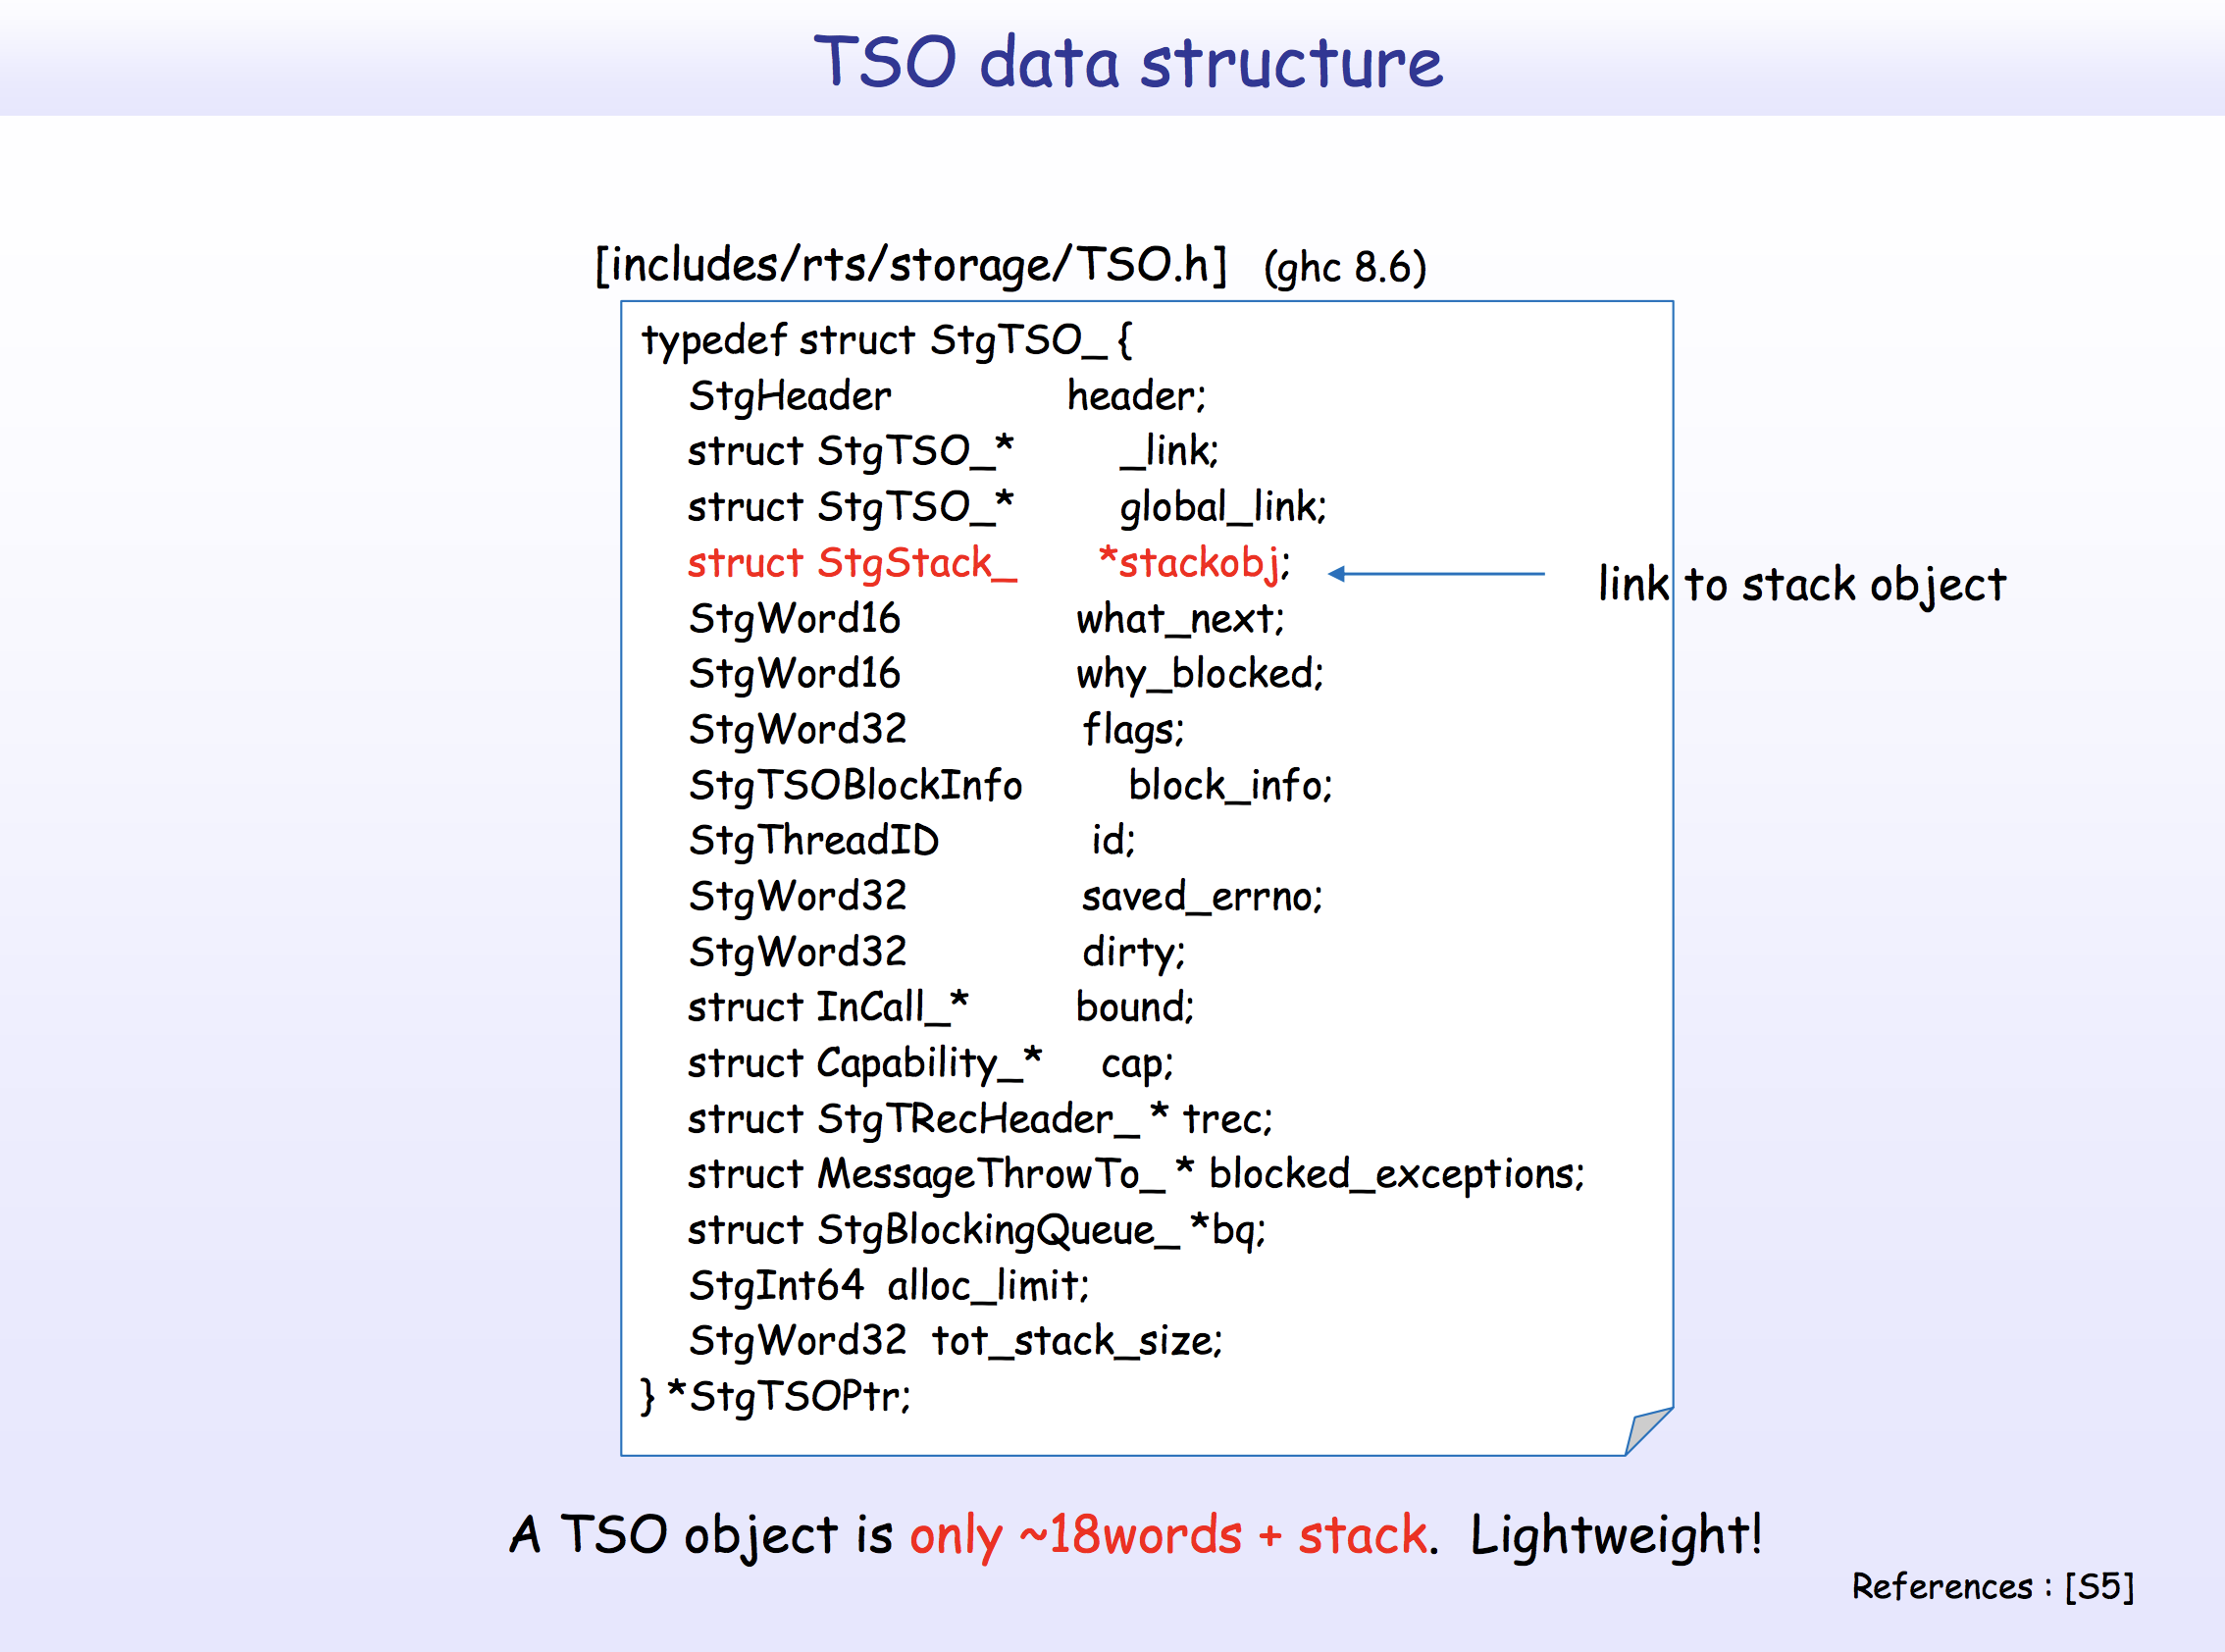
\includegraphics[width=.7\textwidth]{pic/tso.png}
  \footnote{Reference: takenobu-hs, ``haskell-ghc-illustrated'' - \url{https://takenobu-hs.github.io/downloads/haskell_ghc_illustrated.pdf}}
\end{frame}

\end{document}
